In this section we include two plots that summarizes the results obtained when validating the final models in both development and hold-out set.

\begin{figure}[H]
	\centering
	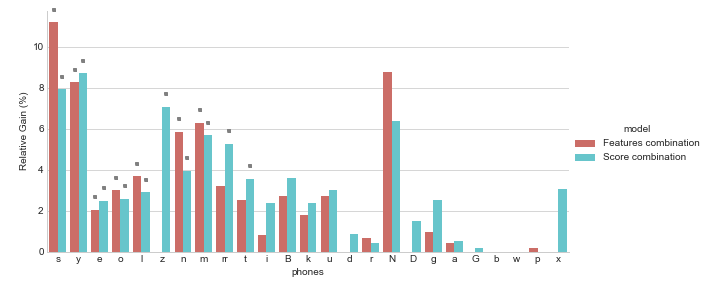
\includegraphics[width=0.8\textwidth]{files/figures/results/relatives/relatives-fusion-systems-dev-all.png}
	\caption{Comparison of relative gains over the Baseline Systems
	between Features Combination systems and Score Combination systems
	computed on the development set for all the phones.
	Results are sorted in descending order according to their
	McNemar p-values computed on the development set.
	Only the results marked with (*) gave statistically significant gains in the development set.}
	\label{fig:fusionAllDev}
\end{figure}

\begin{figure}[H]
	\centering
	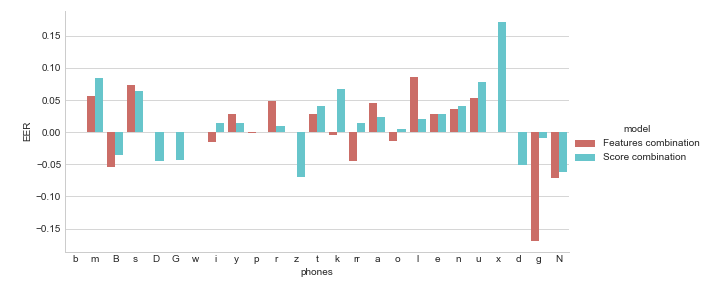
\includegraphics[width=0.8\textwidth]{files/figures/results/relatives/relative-fusion-systems-heldout-all.png}
	\caption{
		Comparison of relative gains over the Baseline Systems
		between Features Combination systems and Score Combination systems
		computed on the hold-out set for all the phones.
		Results are sorted in descending order according to their
		McNemar p-values computed on the development set.
		Only the results marked with (*) gave statistically significant gains in the development set.
	}
	\label{fig:fusionAllHeldout}
\end{figure}
